\section{Hartley}\label{hartley}

Tags: PC Creatore: Lorenzo Giocatore: Lorenzo Luogo: Azura Razza:
Tiefling Classe: Ladro, Mastermind Livello: 10

\section{Hartley}\label{hartley-1}

\begin{center}\rule{0.5\linewidth}{0.5pt}\end{center}

\begin{figure}
\centering
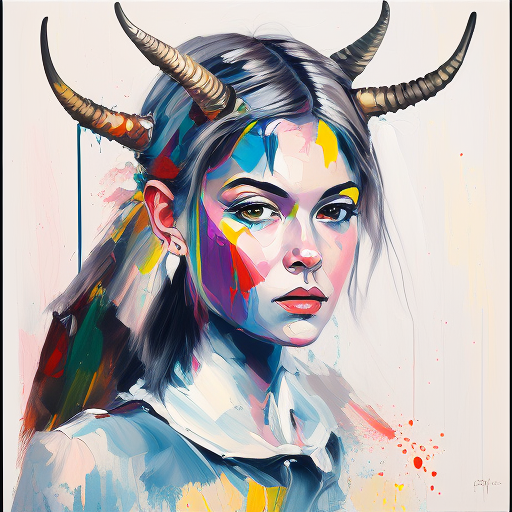
\includegraphics{Hartley_autoritratto.png}
\caption{Hartley\_autoritratto.png}
\end{figure}

Informazioni Generali

Età: 25

Anno di nascita: 1998

Paese di nascita: Kos

Razza: Tiefling

Relazioni:

Alleati:

Nemesi:

Possedimenti importanti:

\begin{center}\rule{0.5\linewidth}{0.5pt}\end{center}

\subsection{1. Descrizione Generale}\label{descrizione-generale}

\begin{center}\rule{0.5\linewidth}{0.5pt}\end{center}

\begin{figure}
\centering
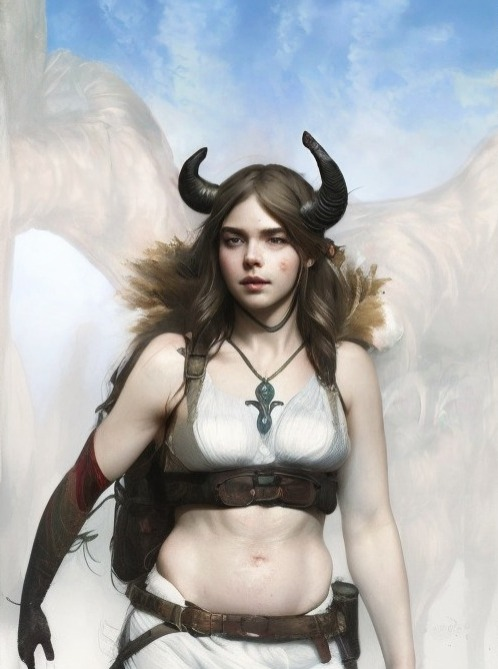
\includegraphics{Hartley.jpeg}
\caption{Hartley.jpeg}
\end{figure}

Lettera di risposta di Marpalo (Quartiermastro dei Protettori di Kos)
alla richiesta di Sitahu di inviare ad Azura un protettore adatto ad una
missione di spionaggio.

``Come mi hai chiesto, ecco tutto quello che so su Hartley Nessuno
conosce la sua vera storia, perché racconta una cosa diversa ogni volta
che qualcuno gliela chiede. A volte è scappata dall'estremo Nord a causa
delle persecuzioni contro i tiefling, altre volte è un'ex prostituta che
ha dovuto uccidere il suo pappone per conquistare la propria libertà,
altre ancora una principessa scappata dal massacro della sua famiglia
durante le rivolte popolari di chissà quale regno lontano. Non
conosciamo neanche il suo cognome, in tasca ha sempre più di un
documento pronto a testimoniare in favore delle sue molteplici
personalità. Probabilmente neanche lei si ricorda più come si chiama.
Bugiarda patologica, ma convincente, mente anche quando non c'è alcun
motivo valido per farlo. Il problema più grande è il suo modo di fare:
sempre cordiale, di buon umore, pronta ad ascoltare e a compatire.
Diresti di lei che è la tua amica più fidata, almeno fino a quando non
riesce ad ottenere da te quello di cui aveva bisogno. Di lei sappiamo
solo che si guadagnava da vivere per strada, distraendo i passanti con
giochi di prestigio e derubandoli mentre lo faceva. Alla fine dello
spettacolo le lasciavano anche qualche monetina (se non le aveva già
prese)! Col passare del tempo ha alzato il tiro, arrivando a svaligiare
le case e gli appartamenti dei cittadini più ambienti della città, fino
a quando non ha fatto il passo più lungo della gamba. Ha deciso di
introdursi nella casa di noto politico Kosentino, uno degli uomini più
influenti di Kos, con una delle case più sorvegliate della città. È
riuscita ad entrare senza fatica, e di questo le bisogna dare merito, ma
non è più uscita. Dopo essere stata catturata avrebbe potuto finire il
resto dei suoi giorni in galera, ma per sua fortuna il suo bersaglio è
anche uno dei principali benefattori della Gilda dei Protettori, e le ha
proposto di mettere le sue capacità al servizio dei bisognosi, lavorando
per la Gilda. In cambio avrebbe fatto decadere tutte le accuse che
gravavano sulla sua testa. Ancora ci chiediamo come sia possibile che le
abbia concesso una grazia del genere, probabilmente è caduto vittima dei
suoi incantesimi da manipolatrice! È stata scortata alla Gilda dalle
guardie cittadine, che hanno presidiato la nostra sede per poco più di
una settimana, poi sono sparite. Hartley da allora è con noi, anche se
adesso potrebbe scappare con il nostro equipaggiamento e spacciarsi per
una Protettrice. Si è rivelata un'ottima risorsa in più di una missione,
riesce ad a trovare una soluzione anche nelle situazioni più difficili,
e non c'è serratura che riesca a fermarla. Tuttavia si rifiuta di
combattere, non si abbassa a ``barbarie del genere'', come dice spesso.
``Le giuste parole aprono più teste di una scure'' dice anche. Spero che
queste informazioni ti possano essere utili nella scelta dei componenti
per la tua squadra. Porta i miei saluti alla tua Francine e ai piccoli
Tuo Marpalo''

\begin{center}\rule{0.5\linewidth}{0.5pt}\end{center}

\subsection{2. Coinvolgimenti in eventi
recenti}\label{coinvolgimenti-in-eventi-recenti}

\begin{center}\rule{0.5\linewidth}{0.5pt}\end{center}

\href{Untitled\%20Database\%20f0a0837cffd44ac7a9471133f60c97b8.csv}{Untitled
Database}

\subsection{6. Scheda personaggio}\label{scheda-personaggio}

\begin{center}\rule{0.5\linewidth}{0.5pt}\end{center}

\href{Info\%20PG\%20792973e9c98e424b8fa1da3d1c2eeac4.csv}{Info PG}

\subsubsection{Statistiche e abilità}\label{statistiche-e-abilituxe0}

\begin{center}\rule{0.5\linewidth}{0.5pt}\end{center}

\href{Abilita\%CC\%80\%207db3a6b653ad434187ea54a65d788929.csv}{Abilità}

\subsubsection{Lista magie}\label{lista-magie}

\subsection{A. Descrizione originale}\label{a.-descrizione-originale}

\begin{center}\rule{0.5\linewidth}{0.5pt}\end{center}
